\documentclass[12pt]{article}

\usepackage[utf8]{inputenc}
\usepackage{datetime}
\usepackage{amsthm}
\usepackage{amsmath}
\usepackage{amssymb}
\usepackage{enumitem}
\usepackage[american]{babel}
\usepackage{matlab-prettifier}
\usepackage{graphicx}
\usepackage[makeroom]{cancel}
\usepackage{afterpage}
\usepackage{capt-of}
\usepackage{bm}

\DeclareMathOperator*{\argmin}{arg\,min}
\DeclareMathOperator*{\argmax}{arg\,max}

\newcommand\independent{\protect\mathpalette{\protect\independenT}{\perp}}
\def\independenT#1#2{\mathrel{\rlap{$#1#2$}\mkern2mu{#1#2}}}

\newtheoremstyle{colon}{\topsep}{\topsep}{}{}{\bfseries}{:}{ }{}
\theoremstyle{colon}
\newtheorem{exercise}{Exercise}
\newtheorem*{answer}{Answer}

\title{ELE 538: Large-Scale Optimization \\ Homework 3}
\author{Zachary Hervieux-Moore}

\newdate{date}{25}{4}{2018}
\date{\displaydate{date}}

\begin{document}

\maketitle

\clearpage

\begin{exercise}
	\textbf{Smoothness:}
	\begin{enumerate}[label=\alph*)]
		\item Show that $f_\mu (\bm{x}) := \sqrt{\lVert \bm{x} \rVert_2^2 + \mu^2} - \mu$ is $\frac{1}{\mu}$-smooth.
		\item Show that $f_\mu (\bm{x}) = \mu \log(\sum_{i=1}^n e^{x_i/\mu}) - \mu \log(n)$ $(\bm{x} \in \mathbb{R}^n)$ is $\frac{1}{\mu}$-smooth.
	\end{enumerate}
\end{exercise}

\begin{answer}
	\
	\begin{enumerate}[label=\alph*)]
		\item Let $g(\bm{x}) = \sqrt{\lVert \bm{x} \rVert_2^2 + \mu^2}$, then we have
			\begin{gather*}
				\nabla f_\mu (\bm{x}) = \frac{\bm{x}}{g(\bm{x})} \\
				\nabla^2 f_\mu(\bm{x}) = \frac{1}{g(\bm{x})} I - \frac{\bm{x} \bm{x}^T}{g(\bm{x})^3}
			\end{gather*}
			Since $I$ and $\bm{x} \bm{x}^T$ commute, then the eigenvalues of their sum is simply the sum of their individual eigenvalues. Also, $\bm{x} \bm{x}^T$ only has one non-zero eigenvalue, namely $\lVert \bm{x} \rVert_2^2$. Therefore, the eigenvalues have the form
			\begin{gather*}
				\frac{1}{g(\bm{x})} - \frac{\lVert \bm{x} \rVert_2^2}{g(\bm{x})^3}  = \frac{\mu^2}{g(\bm{x})^3}\\ 
				\text{ or } \frac{1}{g(\bm{x})}
			\end{gather*}
			Note that these are always positive. Maximizing either of these can be accomplished via simple calculus, we can treat $\lVert \bm{x} \rVert_2^2$ as a univariable,
			\begin{gather*}
				\max_{\bm{x}} \frac{\mu^2}{(\lVert \bm{x} \rVert_2^2 + \mu^2)^{3/2}} = \frac{1}{\mu} \\
				\text{ or } \max_{\bm{x}} \frac{1}{\sqrt{\lVert \bm{x} \rVert_2^2 + \mu^2}} = \frac{1}{\mu}
			\end{gather*}
			We conclude that $\nabla^2 f_\mu(\bm{x}) \preceq \frac{1}{\mu} \bm{I}$

		\item Let $y = \sum_{i=1}^n e^{x_i/\mu}$, then we have
			\begin{gather*}
				[ \nabla f_\mu (\bm{x}) ]_i = \frac{e^{x_i/\mu}}{y} \\
				[ \nabla^2 f_\mu (\bm{x}) ]_{ij} = \begin{cases}
					\frac{\frac{1}{\mu} (e^{x_i/\mu}y - e^{2x_i/\mu})}{y^2}, \text{ if } i = j \\
					\frac{-\frac{1}{\mu} e^{x_i/\mu + x_j/\mu}}{y^2}, \text{ if } i \neq j
				\end{cases}
			\end{gather*}
			In matrix form, letting $\bm{z} = [e^{x_1/\mu} \ \cdots \ e^{x_n/\mu}]$
			\begin{gather*}
				\nabla^2 f_\mu (\bm{x}) = \frac{1}{\mu y} \text{diag}(e^{x_1/\mu}, \mathellipsis, e^{x_n/\mu}) - \frac{1}{\mu y^2} \bm{z} \bm{z^T}
			\end{gather*}
			We again have two commuting matrices with the subtrahend being an outer product. Again, using the facts we used in part a), we get that the eigenvalues have the form
			\begin{gather*}
				\frac{1}{\mu y} e^{x_i/\mu} - \frac{1}{\mu y^2} \lVert \bm{z} \rVert_2^2 \\
				\text{ or } \frac{1}{\mu y} e^{x_i/\mu}
			\end{gather*}
			Where we note that $y^2 \geq \lVert \bm{z} \rVert_2^2$ and so the eigenvalues are all non-negative. Furthermore, the maximal eigenvalue must come from the second form of eigenvalue. Then maximizing the second line above, with relatively simple calculus, we have that picking $y = e^{x_i/\mu}$, that is, $x_i = c, x_j \rightarrow -\infty \ \forall i \neq j$ is the maximizer. Thus,
			\begin{gather*}
				\sup_{\bm{x}} \frac{1}{\mu y} e^{x_i/\mu} = \frac{1}{\mu}
			\end{gather*}
			We conclude that $\nabla^2 f_\mu(\bm{x}) \preceq \frac{1}{\mu} \bm{I}$
	\end{enumerate}
\end{answer}

\clearpage

\begin{exercise}
	\textbf{Nesterov's coefficient:} Recall that one version of Nesterov's momentum coefficients is generated by
	\begin{gather*}
		\theta_{t+1} = \frac{1 + \sqrt{1 + 4 \theta_t^2}}{2}
	\end{gather*}
	with $\theta_0 = 1$.
	\begin{enumerate}[label=\alph*)]
		\item Show that for all $t \geq 1$, one has $\theta_t \geq \frac{t+2}{2}$.
		\item Show that
			\begin{gather*}
				\frac{\theta_t - 1}{\theta_{t+1}} = 1 - \frac{3}{t} + o(\frac{1}{t})
			\end{gather*}
	\end{enumerate}
\end{exercise}

\begin{answer}
	\
	\begin{enumerate}[label=\alph*)]
		\item This is a simple proof by induction. Clearly, it is true for $\theta_0 = 1 \geq \frac{2}{2} = 1$. Now for the induction step,
			\begin{align*}
				\theta_{t+1} &= \frac{1 + \sqrt{1 + 4\theta_t^2}}{2} \\
				&\geq \frac{1 + \sqrt{1 + (t+2)^2}}{2} \quad \text{ by induction hypothesis} \\
				&\geq \frac{\sqrt{(t+2)^2}}{2} \quad \text{ by making the numerator smaller} \\
				&\geq \frac{t+2}{2}
			\end{align*}

		\item We begin by just using definitions and manipulating
			\begin{align*}
				\frac{\theta_t - 1}{\theta_{t+1}} &= \frac{2 \theta_t - 2}{1 + \sqrt{1 + 4 \theta_t^2}} \\
				&= \frac{(2 \theta_t - 2)(\sqrt{1 + 4 \theta_t^2} - 1)}{4 \theta_t^2} \\
				&= \frac{(\theta_t - 1)(\sqrt{1 + 4 \theta_t^2} - 1)}{2 \theta_t^2}
			\end{align*}
			Now, calculating the Laurent series of the above yields
			\begin{gather*}
				\frac{\theta_t - 1}{\theta_{t+1}} = 1 - \frac{3}{2 \theta_t} + o \left( \frac{1}{\theta_t} \right)
			\end{gather*}
			Now, by part a), we know that $\frac{1}{\theta_t} = \frac{2}{t+2} + o \left( \frac{1}{t} \right) = \frac{2}{t} + o \left( \frac{1}{t} \right)$, which concludes the proof.
	\end{enumerate}
\end{answer}

\clearpage

\begin{exercise}
	\textbf{Infimal convolution:} Define the infimal convolution of two functions $f$ and $g$ as
	\begin{gather*}
		(f \square g)(\bm{x}) := \inf_{\bm{y}} \{ f(\bm{y}) + g(\bm{x} - \bm{y}) \}
	\end{gather*}
	with $\theta_0 = 1$.
	\begin{enumerate}[label=\alph*)]
		\item Show that the Fenchel conjugate obeys $(f \square g)^* = f^* + g^*$
		\item Suppose $f$ is convex. Use part a) to show that the Moreau envelope $M_{\mu f}(\bm{x}) := \inf_{\bm{z}} \{ f(\bm{z}) + \frac{1}{2\mu} \lVert \bm{x} - \bm{z} \rVert_2^2 \}$ is $\frac{1}{\mu}$-smooth.
	\end{enumerate}
	\textbf{Hint: } if a function $f$ is $\alpha$-strongly convex, then $f^*$ is $\frac{1}{\alpha}$-smooth.
\end{exercise}

\begin{answer}
	\
	\begin{enumerate}[label=\alph*)]
		\item By definition of the Fenchel conjugate,
			\begin{gather*}
				(f \square g)^*(\bm{\theta}) = \sup_{\bm{x}} \left\{ \langle \bm{x}, \bm{\theta} \rangle - \inf_{\bm{y}} \{ f(\bm{y}) + g(\bm{x}-\bm{y}) \} \right\} \\
				= \sup_{\bm{x}} \left\{ \langle \bm{x}, \bm{\theta} \rangle + \sup_{\bm{y}} \{ - f(\bm{y}) - g(\bm{x}-\bm{y}) \} \right\} \\
				= \sup_{\bm{x}, \bm{y}} \{ \langle \bm{x}, \bm{\theta} \rangle - f(\bm{y}) - g(\bm{x}-\bm{y}) + \langle \bm{y}, \bm{\theta} \rangle - \langle \bm{y}, \bm{\theta} \rangle \} \\
				= \sup_{\bm{x}, \bm{y}} \{ \langle \bm{y}, \bm{\theta} \rangle - f(\bm{y}) + \langle \bm{x} - \bm{y}, \bm{\theta} \rangle - g(\bm{x}-\bm{y}) \} \\
				= \sup_{\bm{y}} \{ \langle \bm{y}, \bm{\theta} \rangle - f(\bm{y}) \} + \sup_{\bm{z}} \{ \langle \bm{z}, \bm{\theta} \rangle - g(\bm{z}) \} \\
				= f^*(\bm{\theta}) + g^*(\bm{\theta})
			\end{gather*}
			Where the substitution $\bm{z} = \bm{x} - \bm{y}$ is valid because $\bm{z}$ can still span all $\mathbb{R}^n$ for fixed $\bm{y}$.

		\item Given, $M_{\mu f}(\bm{x}) := \inf_{\bm{z}} \{ f(\bm{z}) + \frac{1}{2\mu} \lVert \bm{x} - \bm{z} \rVert_2^2 \}$, we let $g(\bm{x}) = \frac{1}{2\mu} \lVert \bm{x}\rVert_2^2$, then we have precisely that
			\begin{gather*}
				M_{\mu f}(\bm{x}) = (f \square g)(\bm{x})
			\end{gather*}
			Using the hint, we calculate the Fenchel conjugate of the above by using part a),
			\begin{gather*}
				M_{\mu f}^*(\bm{x}) = f^*(\bm{x}) + g^*(\bm{x})
			\end{gather*}
			Now, we calculate $g^*$,
			\begin{gather*}
				g^*(\bm{\theta}) = \sup_{\bm{x}} \{ \langle \bm{x}, \bm{\theta} \rangle - \frac{1}{2\mu} \lVert \bm{x} \rVert_2^2 \}
			\end{gather*}
			Taking the gradient and setting to $0$ yields
			\begin{gather*}
				\nabla \implies \bm{\theta} - \frac{1}{\mu} \bm{x} = 0 \implies \bm{x} = \mu \bm{\theta}
			\end{gather*}
			So,
			\begin{gather*}
				g^*(\bm{\theta}) = \frac{\mu}{2} \lVert \bm{\theta} \rVert_2^2
			\end{gather*}
			and
			\begin{gather*}
				M_{\mu f}^*(\bm{x}) = f^*(\bm{x}) + \frac{\mu}{2} \lVert \bm{x} \rVert_2^2
			\end{gather*}
			As $f^*$ is convex, then we have that $M_{\mu f}^*(\bm{x})$ is $\mu$-strongly convex by definition. Then, by the hint, we have $M_{\mu f}(\bm{x})$ is $\mu$-smooth.
	\end{enumerate}
\end{answer}

\clearpage

\begin{exercise}
	\textbf{Moreau envelope:} Let $f$ be a convex function.
	\begin{enumerate}[label=\alph*)]
		\item Suppose that the Moreau envelope $M_f(\bm{x}) > -\infty$ for all $\bm{x}$. Show that $M_f(\cdot)$ is convex.
		\item Show that $\nabla M_{\mu f}(\bm{x}) = \frac{1}{\mu} (\bm{x} - \text{prox}_{\mu f}(\bm{x}))$.
		\item Show that $\text{prox}_f(\bm{x}) = \nabla M_{f^*} (\bm{x})$
	\end{enumerate}
\end{exercise}

\begin{answer}
	\
	\begin{enumerate}[label=\alph*)]
		\item Using the standard definition of convexity
			\begin{gather*}
				M_f(\lambda \bm{x} + (1-\lambda) \bm{y}) = \inf_{\bm{z}} \{ f(\bm{z}) + \frac{1}{2} \lVert \lambda \bm{x} + (1-\lambda) \bm{y} - \bm{z} \rVert_2^2 \} \\
				= \inf_{\bm{z}_1, \bm{z}_2} \{ f(\lambda \bm{z}_1 + (1-\lambda)\bm{z}_2) + \frac{1}{2} \lVert \lambda \bm{x} -  (1-\lambda) \bm{y} - \lambda \bm{z}_1 - (1-\lambda)\bm{z}_2 \rVert_2^2 \}
			\end{gather*}
			Where the infimum is not changed because one can pick $\bm{z} = \lambda \bm{z}_1^* + (1-\lambda)\bm{z}_2^*$. Using convexity of $f$ and triangle inequality,
			\begin{align*}
				&\leq \inf_{\bm{z}_1, \bm{z}_2} \{ \lambda f(\bm{z}_1) + \frac{1}{2} \lVert \lambda \bm{x} - \lambda \bm{z}_1 \rVert_2^2 \\
				&\quad + (1-\lambda) f(\bm{z}_2) + \frac{1}{2} \lVert (1-\lambda) \bm{y} - (1-\lambda) \bm{z}_2 \rVert_2^2 \}
			\end{align*}
			Since $\lambda \in (0,1)$ we get,
			\begin{gather*}
				\leq \inf_{\bm{z}_1, \bm{z}_2} \{ \lambda f(\bm{z}_1) + \frac{\lambda}{2} \lVert \bm{x} - \bm{z}_1 \rVert_2^2 + (1-\lambda) f(\bm{z}_2) + \frac{(1-\lambda)}{2} \lVert  \bm{y} - \bm{z}_2 \rVert_2^2 \} \\
				= \lambda M_f(\bm{x}) + (1-\lambda) M_f(\bm{y})
			\end{gather*}
			
		\item We have that
			\begin{gather*}
				M_{\mu f} (\bm{x}) = \inf_{\bm{z}} \{ f(\bm{z}) + \frac{1}{2\mu} \lVert \bm{x} - \bm{z} \rVert_2^2 \} \\
				= - \sup_{\bm{z}} \{ -f(\bm{z}) - \frac{1}{2\mu} \lVert \bm{x} - \bm{z} \rVert_2^2 \} \\
				= - \sup_{\bm{z}} \{ -f(\bm{z}) - \frac{1}{2\mu} \lVert \bm{x} \rVert_2^2 + \frac{1}{\mu} \langle \bm{x}, \bm{z} \rangle - \frac{1}{2\mu} \lVert \bm{z}\rVert_2^2 \} \\
				= \frac{1}{2\mu} \lVert \bm{x} \rVert_2^2 - \frac{1}{\mu} \sup_{\bm{z}} \{ \langle \bm{x}, \bm{z} \rangle - \mu f(\bm{z}) - \frac{1}{2} \lVert \bm{z}\rVert_2^2 \} \\
			\end{gather*}
			Define $g(\bm{z}) = \mu f(\bm{z}) + \frac{1}{2} \lVert \bm{z}\rVert_2^2$ to get
			\begin{gather*}
				M_{\mu f} (\bm{x}) = \frac{1}{2\mu} \lVert \bm{x} \rVert_2^2 - \frac{1}{\mu} g^*(\bm{x})
			\end{gather*}
			Thus, we have
			\begin{gather*}
				\nabla M_{\mu f} (\bm{x}) = \frac{1}{\mu} (\bm{x} - \nabla g^*(\bm{x}))
			\end{gather*}
			Thus, we just have to show that $\nabla g^*(\bm{x}) = \text{prox}_{\mu f}(\bm{x})$. Since
			\begin{gather*}
				g^*(\bm{x}) = \sup_{\bm{z}} \{ \langle \bm{x}, \bm{z} \rangle - \mu f(\bm{z}) - \frac{1}{2} \lVert \bm{z}\rVert_2^2 \}
			\end{gather*}
			Suppose that $\bm{z}^*$ is the supremum, then 
			\begin{gather*}
				g^*(\bm{x}) = \langle \bm{x}, \bm{z}^* \rangle - \mu f(\bm{z}^*) - \frac{1}{2} \lVert \bm{z}^* \rVert_2^2 \\
				\implies \nabla g^*(\bm{x}) = \bm{z}^* \\
				= \argmax_{\bm{z}} \{ \langle \bm{x}, \bm{z} \rangle - \mu f(\bm{z}) - \frac{1}{2} \lVert \bm{z}\rVert_2^2 \} \\
				= \argmin_{\bm{z}} \{ f(\bm{z}) + \frac{1}{2\mu} \lVert \bm{z} \rVert_2^2 - \frac{1}{\mu} \langle \bm{x}, \bm{z} \rangle \}
			\end{gather*}
			Adding the scalar $\frac{1}{2\mu} \lVert \bm{x}\rVert_2^2$ does not change the $\argmax$
			\begin{gather*}
				g^*(\bm{x}) = \argmin_{\bm{z}} \{ f(\bm{z}) + \frac{1}{2\mu} \lVert \bm{z} \rVert_2^2 - \frac{1}{\mu} \langle \bm{x}, \bm{z} \rangle + \frac{1}{2\mu} \lVert \bm{z} \rVert_2^2 \} \\
				= \{ f(\bm{z}) + \frac{1}{2\mu} \lVert \bm{x} - \bm{z} \rVert_2^2 \} \\
				= \text{prox}_{\mu f}(\bm{x})
			\end{gather*}
			Thus, we have shown what we wanted to show.

		\item From the previous part, we have
			\begin{gather*}
				\nabla M_{f^*} (\bm{x}) = \bm{x} - \text{prox}_{f^*}(\bm{x})
			\end{gather*}
			By Moreau's decomposition, we have $\bm{x} - \text{prox}_{f^*}(\bm{x}) = \text{prox}_{f}(\bm{x})$. We conclude
			\begin{gather*}
				\nabla M_{f^*} (\bm{x}) = \text{prox}_{f}(\bm{x})
			\end{gather*}
	\end{enumerate}
\end{answer}

\clearpage

\begin{exercise}
	\textbf{ADMM and consensus optimization:} The general form ADMM problem is
	\begin{gather*}
		\min f(\bm{x}) + h(\bm{z}) \\
		\text{s.t. } \bm{A} \bm{x} + \bm{B} \bm{z} = \bm{b}
	\end{gather*}
	with variables $\bm{x} \in \mathbb{R}^n$, $\bm{z} \in \mathbb{R}^m$. Assume that both $f$ and $h$ are convex, and assume $\bm{b} \in \mathbb{R}^p$ (i.e., there are $p$ scalar equality constraints).

	A special case is the $(two variable)$ consensus problem, which has the form
	\begin{gather*}
		\min f(\bm{x}) + h(\bm{z}) \\
		\text{s.t. } \bm{x} - \bm{z} = \bm{0}
	\end{gather*}
	Show how to reduce the general form ADMM problem to the consensus problem. (In other words, explain how to solve the general form problem, assuming you can solve the solve the consensus problem). Explain why the functions in your consensus problem are convex. (You do not have to worry about analysis details, such as showing that functions are closed). Explain the relation between ADMM for the general form problem and ADMM for the consensus problem that you form in your reduction.

	\textbf{Hint: } define $\tilde{f}(\tilde{\bm{x}}) = \inf_{\bm{A}\bm{x} = \tilde{\bm{x}}} f(\bm{x})$.
\end{exercise}

\begin{answer}
	We transform the general ADMM into the consensus problem by making the substitutions $\tilde{f}(\tilde{\bm{x}}) = \inf_{\bm{A}\bm{x} = \tilde{\bm{x}}} f(\bm{x})$ and $\tilde{h}(\tilde{\bm{z}}) = \inf_{\bm{b} - \bm{B}\bm{z} = \tilde{\bm{z}}} h(\bm{z})$. These are convex functions because
	\begin{gather*}
		\tilde{f}(\lambda \tilde{\bm{x}}_1 + (1-\lambda) \tilde{\bm{x}}_2) = \inf_{\bm{A}\bm{x} = \lambda \tilde{\bm{x}}_1 + (1-\lambda) \tilde{\bm{x}}_2} f(\bm{x}) \\ 
		= \inf_{\bm{A}(\lambda \bm{x}_1 + (1-\lambda) \bm{x}_2) = \lambda \tilde{\bm{x}}_1 + (1-\lambda) \tilde{\bm{x}}_2} f(\lambda \bm{x}_1 + (1-\lambda) \bm{x}_2)
	\end{gather*}
	Where the substitution $\bm{x} = \lambda \bm{x}_1 + (1-\lambda) \bm{x}_2)$ is valid because picking $\bm{x} = \lambda \bm{x}_1^* + (1-\lambda) \bm{x}_2^*$ (the respective infima) is feasible in the original infimum. Now using convexity of $f$
	\begin{gather*}
		\leq \inf_{\bm{A}(\lambda \bm{x}_1 + (1-\lambda) \bm{x}_2) = \lambda \tilde{\bm{x}}_1 + (1-\lambda) \tilde{\bm{x}}_2} \lambda f(\bm{x}_1) + (1-\lambda) f(\bm{x}_2) \\
		\leq \inf_{\substack{\bm{A} \bm{x}_1 = \tilde{\bm{x}}_1 \\ \bm{A} \bm{x}_2 = \tilde{\bm{x}}_2}} \lambda f(\bm{x}_1) + (1-\lambda) f(\bm{x_2})
	\end{gather*}
	Where the second inequality holds because the new problem is more restrictive. Finally, we conclude $\tilde{f}(\tilde{\bm{x}})$ is convex with:
	\begin{gather*}
		= \inf_{\bm{A} \bm{x}_1 = \tilde{\bm{x}}_1} \lambda f(\bm{x}_1) + \inf_{\bm{A} \bm{x}_2 = \tilde{\bm{x}}_2}  (1-\lambda) f(\bm{x_2}) \\
		= \lambda \tilde{f}(\tilde{\bm{x}}_1) + (1-\lambda) \tilde{f}(\tilde{\bm{x}}_2)
	\end{gather*}

	$\tilde{h}(\tilde{\bm{z}})$ is convex by similar logic. Using these substitutes, the problem becomes
	\begin{gather*}
		\min \tilde{f}(\tilde{\bm{x}}) + \tilde{h}(\tilde{\bm{z}}) \\
		\text{s.t. } \tilde{\bm{x}} - \tilde{\bm{z}} = 0
	\end{gather*}

	For completeness, the original ADMM updates are:
	\begin{gather*}
		\bm{x}^{t+1} = \argmin_{\bm{x}} \{ f(\bm{x}) + \frac{\rho}{2} \lVert \bm{A} \bm{x} + \bm{B} \bm{z}^t - \bm{b} + \frac{1}{\rho} \bm{\lambda}^t \rVert_2^2 \} \\
		\bm{z}^{t+1} = \argmin_{\bm{z}} \{ h(\bm{z}) + \frac{\rho}{2} \lVert \bm{A} \bm{x}^{t+1} + \bm{B} \bm{z} - \bm{b} + \frac{1}{\rho} \bm{\lambda}^t \rVert_2^2 \} \\
		\bm{\lambda}^{t+1} = \bm{\lambda}^t + \rho (\bm{A} \bm{x}^{t+1} + \bm{B} \bm{z}^{t+1} - \bm{b})
	\end{gather*}

	While the consensus problem's is:
	\begin{gather*}
		\tilde{\bm{x}}^{t+1} = \argmin_{\tilde{\bm{x}}} \{ \tilde{f}(\tilde{\bm{x}}) + \frac{\rho}{2} \lVert \tilde{\bm{x}} - \tilde{\bm{z}}^t + \frac{1}{\rho} \bm{\lambda}^t \rVert_2^2 \} \\
		\tilde{\bm{z}}^{t+1} = \argmin_{\tilde{\bm{z}}} \{ \tilde{h}(\tilde{\bm{z}}) + \frac{\rho}{2} \lVert \tilde{\bm{x}}^{t+1} - \tilde{\bm{z}} + \frac{1}{\rho} \bm{\lambda}^t \rVert_2^2 \} \\
		\bm{\lambda}^{t+1} = \bm{\lambda}^t + \rho (\tilde{\bm{x}}^{t+1} - \tilde{\bm{z}}^{t+1})
	\end{gather*}

	Notice that the update rules are much simpler on the surface for the consensus problem. However, that is because the $\bm{A}\bm{x} = \tilde{\bm{x}}$ is hidden in $\tilde{f}$. Also, note that the consensus problem is merely the general problem but with $\bm{A} = \bm{I}_n$, $\bm{B} = \bm{I}_m, \bm{b} = \bm{0}$.
\end{answer}

\clearpage

\begin{exercise}
	\textbf{Douglas-Rachford splitting for LP feasibility:}
	\begin{enumerate}[label=\alph*)]
		\item Work out Douglas-Rachford splitting for solving the LP feasibility problem considered in Homework 2, problem 2.
		\item Implement it and report the numerical convergence of $\lVert \bm{x}^t - \bm{x}^{t-\frac{1}{2}} \rVert_2$ vs. $t$. Compare it with alternating projection implemented in HW2.
	\end{enumerate}
\end{exercise}

\begin{answer}
	\
	\begin{enumerate}[label=\alph*)]
		\item To do the Douglas-Rachford splitting, we define the LP feasibility problem as
			\begin{gather*}
				\min_{\bm{x}} f(\bm{x}) + h(\bm{A} \bm{x})
			\end{gather*}
			With $f(\bm{x}) = 1_{\{0 \leq \bm{x}\}}$, the indicator function with $+\infty$ if outside and 0 inside, and $h(\bm{x}) = \frac{1}{2} \lVert \bm{x} - \bm{b} \rVert_2^2$. Which gets turned into the saddle-point problem
			\begin{gather*}
				\min_{\bm{x}} \max_{\bm{\lambda}} f(\bm{x}) + \langle \bm{\lambda}, \bm{A}\bm{x} \rangle + h^*(\bm{\lambda})
			\end{gather*}
			Where
			\begin{gather*}
				h^*(\bm{\lambda}) = \sup_{\bm{z}} \{ \langle \bm{\lambda}, \bm{z} \rangle - \frac{1}{2} \lVert \bm{z} - \bm{b} \rVert_2^2 \} \\
				= \langle \bm{\lambda}, \bm{b} \rangle + \frac{1}{2} \lVert \bm{\lambda} \rVert_2^2
			\end{gather*}
			Where we used the optimality condition $\bm{z} = \bm{b} + \bm{\lambda}$.

			So, all that is left is to compute the proximal operators for $\eta f$ and $\eta h^*$.
			\begin{gather*}
				\text{prox}_{\eta f}(\bm{x}) = \argmin_{\bm{z}} \{ \eta f(\bm{z}) + \frac{1}{2} \lVert \bm{x} - \bm{z} \rVert_2^2 \} \\
				= \argmin_{\bm{z}} \{ \eta 1_{\{0 \leq \bm{z}\}} + \frac{1}{2} \lVert \bm{x} - \bm{z} \rVert_2^2 \}
			\end{gather*}
			Which is trivially satisfied by $\bm{z} = \bm{x}$ if $\bm{x} \geq \bm{0}$. If it is the other case, we must project onto the positive orthant (to get rid of the infinity from the indicator). Thus, we can write it succinctly as
			\begin{gather*}
				\text{prox}_{\eta f}(\bm{x})_i = \max (0, x_i) \quad \forall i
			\end{gather*}

			For $\eta h^*$ we have
			\begin{gather*}
				\text{prox}_{\eta h^*}(\bm{x}) = \argmin_{\bm{z}} \{ \eta h^*(\bm{z}) + \frac{1}{2} \lVert \bm{x} - \bm{z} \rVert_2^2 \} \\
				= \argmin_{\bm{z}} \{ \eta \langle \bm{z}, \bm{b} \rangle + \frac{\eta}{2} \lVert \bm{z} \rVert_2^2 + \frac{1}{2} \lVert \bm{x} - \bm{z} \rVert_2^2 \}
			\end{gather*}
			Optimality conditions yields that $\eta \bm{b} + \eta \bm{z} + \bm{z} - \bm{x} = 0$ or $\bm{z} = \frac{\bm{x} - \eta \bm{b}}{1+\eta}$. Thus,
			\begin{gather*}
				\text{prox}_{\eta h^*}(\bm{x}) = \frac{\bm{x} - \eta \bm{b}}{1+\eta}
			\end{gather*}

			Putting it all together, the Douglas-Rachford splitting is
			\begin{gather*}
				\bm{x}^{t+1/2} = \max (0, p_i^t) \quad \forall i \\
				\bm{\lambda}^{t+1/2} = \frac{\bm{q}^t - \eta \bm{b}}{1+\eta} \\
				\begin{bmatrix}
					\bm{x}^{t+1} \\
					\bm{\lambda}^{t+1}
				\end{bmatrix} = \begin{bmatrix}
					\bm{I} & \eta \bm{A}^T \\
					-\eta \bm{A} & \bm{I}
				\end{bmatrix}^{-1} \begin{bmatrix}
					2 \bm{x}^{t+1/2} - \bm{p}^t \\
					2 \bm{\lambda}^{t+1/2} - \bm{q}^t
				\end{bmatrix} \\
				\bm{p}^{t+1} = \bm{p}^t + \bm{x}^{t+1} - \bm{x}^{t+1/2} \\
				\bm{q}^{t+1} = \bm{q}^t + \bm{\lambda}^{t+1} - \bm{\lambda}^{t+1/2}
			\end{gather*}

		\item The code used to generate the figure is attached below. Figure 1 shows the residual error for alternating projection vs. Douglas-Rachford. Figure 2 shows $\lVert \bm{x}^t - \bm{x}^{t+1/2} \rVert_2$ for both methods. Notice the substantial increase in speed with characteristic ripples

			\begin{center}
		        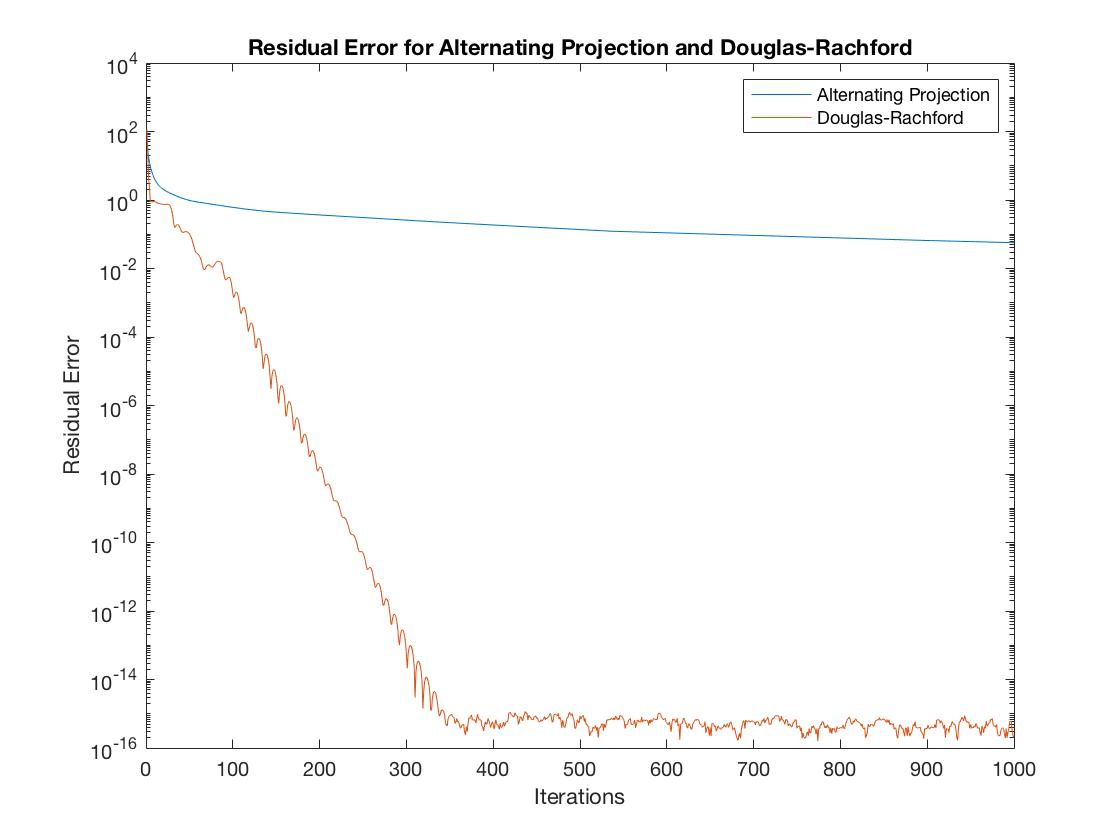
\includegraphics[width=0.8\textwidth]{6b.jpg}
		        \captionof{figure}{Plot of $\lVert \bm{A} \bm{x}^k - \bm{b} \rVert$ for both methods}
			\end{center}

			\begin{center}
		        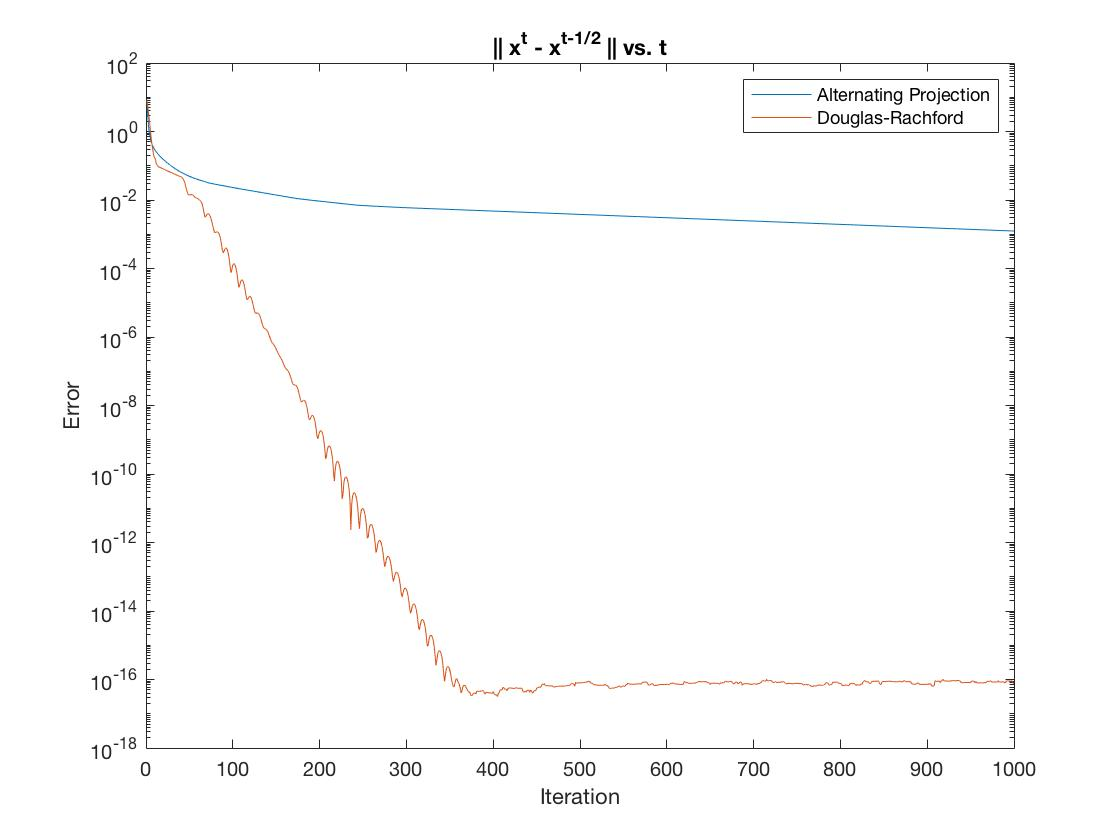
\includegraphics[width=0.8\textwidth]{6c.jpg}
		        \captionof{figure}{Plot of $\lVert \bm{x}^t - \bm{x}^{t+1/2} \rVert_2$ for both methods}
			\end{center}

			\textbf{Code Appendix:}

			\begin{lstlisting}[style=Matlab-editor, basicstyle=\scriptsize]
clear;
clc;

m = 5;
n = 200;

A = rand(m,n);
b = rand(m,1);

% alternating projection
x_ap(:,1) = rand(n,1);
i = 1;
res_ap(1) = norm(x_ap(:,1),2);

while (size(res_ap) < 1000)
    i = i + 1;
    % project into affine set
    x_ap(:,i) = x_ap(:,i-1) + A'/(A*A')*(b-A*x_ap(:,i-1));
    
    i = i + 1;
    % project into positive orthant
    x_ap(:,i) = max(0, x_ap(:,i-1));
    
    % res_ap(ceil(i/2)) = norm(A*x_ap(:,i) - b,2);
    res_ap(ceil(i/2)) = norm(x_ap(:,i) - x_ap(:,i-1),2);
end

% Douglas-Rachford
x_dr = rand(n,1);
lambda_dr = rand(m,1);
p_dr = rand(n,1);
q_dr = rand(m,1);
eta = 0.1;
i = 1;
res_dr(1) = norm(x_dr(:,1),2);

while (size(res_dr) < 1000)
    % project onto positive orthant
    x_dr_half(:,i) = max(0, p_dr(:,i));
    % proximal for norm
    lambda_dr_half(:,i) = (q_dr(:,i) - eta*b)/(1+eta);
    
    % update full step
    tmp = inv([eye(n), eta*A'; -eta*A, eye(m)])*[2*x_dr_half(:,i)-p_dr(:,i);2*lambda_dr_half(:,i)-q_dr(:,i)];
    x_dr(:,i+1) = tmp(1:n);
    lambda_dr(:,i+1) = tmp(n+1:n+m);
    
    % update p and q
    p_dr(:,i+1) = p_dr(:,i) + x_dr(:,i+1) - x_dr_half(:,i);
    q_dr(:,i+1) = q_dr(:,i) + lambda_dr(:,i+1) - lambda_dr_half(:,i);
    
    i = i + 1;
    % res_dr(i) = norm(A*x_dr(:,i) - b,2);
    res_dr(i) = norm(x_dr(:,i) - x_dr_half(:,i-1),2);
end

semilogy(res_ap)
hold on
semilogy(res_dr)
			\end{lstlisting}
	\end{enumerate}
\end{answer}

\end{document}